\begin{withoutheadline}
\begin{frame}
\vspace*{-13mm}
\begin{figure}
	\hspace*{-4.2mm}
    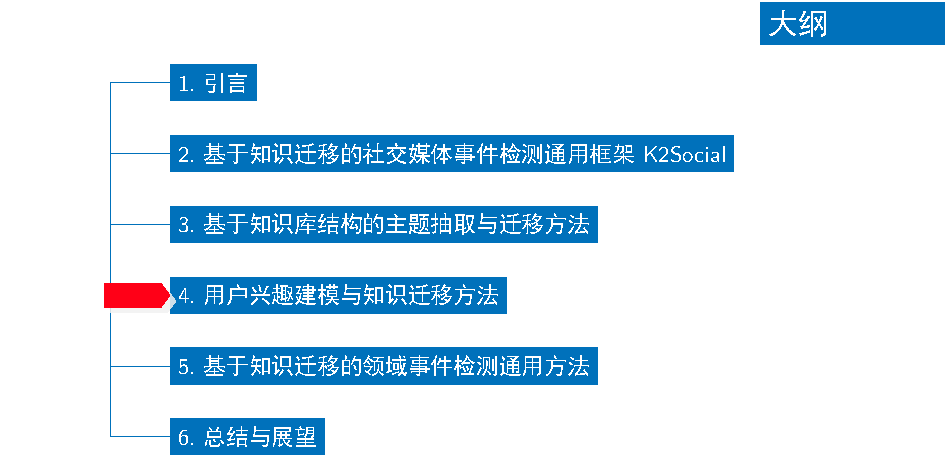
\includegraphics[width=1.0\paperwidth]{img/contents4_output.pdf}
\end{figure}

\end{frame}
\end{withoutheadline}

\section{用户兴趣建模与知识迁移方法}


%TODO 要说明对突发事件检测有迫切需求
\begin{frame}
\frametitle{Motivation}	
issue
说明对突发事件检测有迫切需求

\pdfnote{前面一节中已经分析了知识迁移对事件检测准确性的提升,这一小节中我们分析知识迁移对事件检测时效性的提升}
\end{frame}


\begin{frame}
\frametitle{Motivation}
\begin{figure}[h]
		\setlength{\abovecaptionskip}{0.cm}
        \setlength{\belowcaptionskip}{0.cm}
        \centering
		\caption{社交媒体关注网络用于扩充个人自我描述信息示意图}
        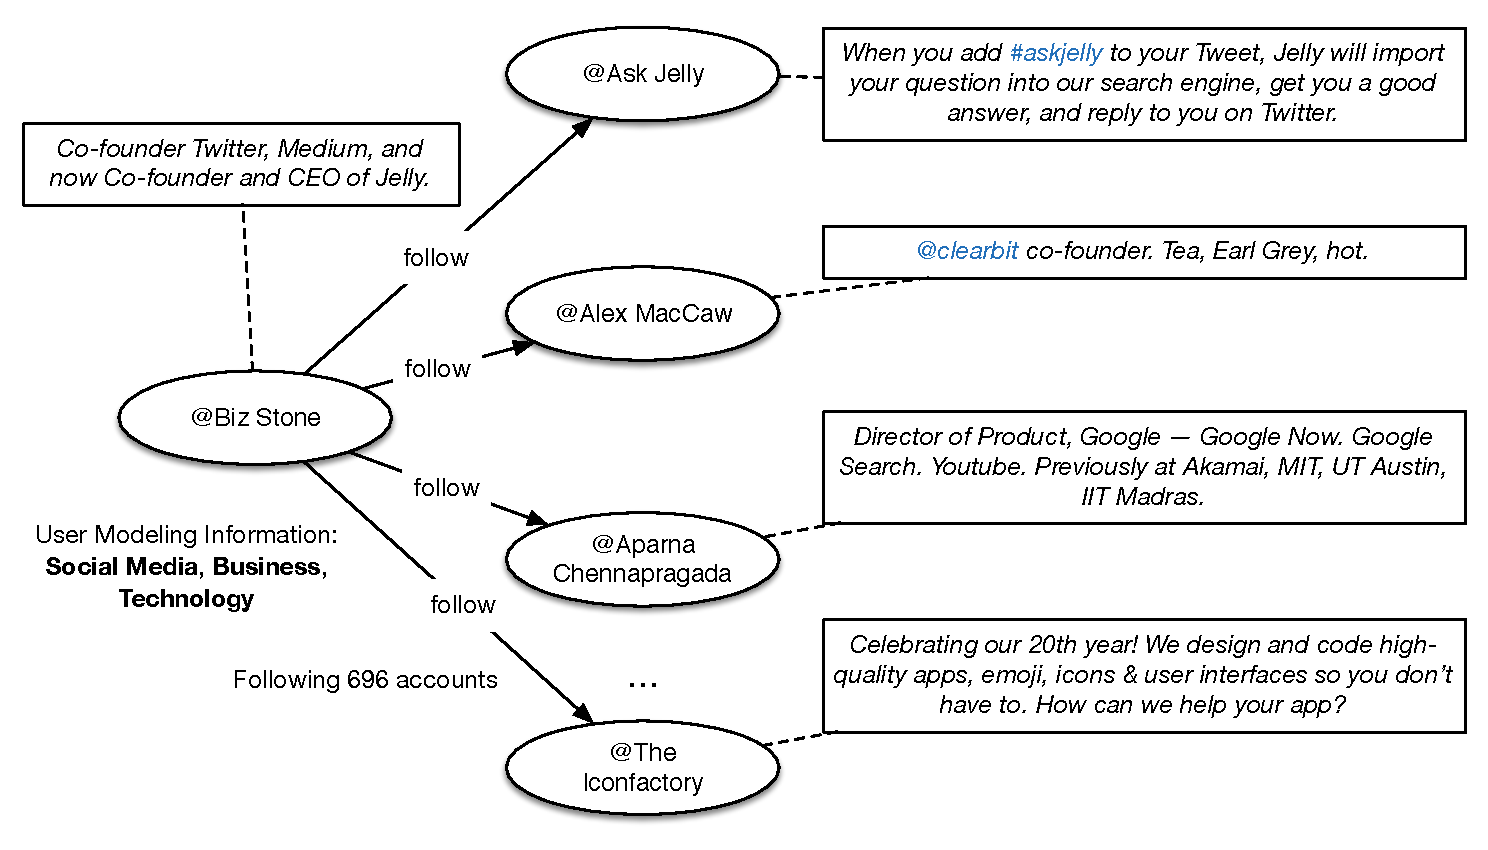
\includegraphics[width=0.9\columnwidth]{img/UMIETM/UMIETM_profile.pdf}
\end{figure}
\end{frame}

